%%%%%%%%%%%%%%%%%%%%%%%%%%%%%%%%%%%%%%%%%%%%%%%%%%%%%%%%%%%%%%%%%%% 
%                                                                 %
%                            CHAPTER FIVE   - Toward a Pasage-Sensitive Agent - Version 3            %
%                                                                 %
%%%%%%%%%%%%%%%%%%%%%%%%%%%%%%%%%%%%%%%%%%%%%%%%%%%%%%%%%%%%%%%%%%% 
 
\chapter{Version 3 -- A Passage-Discerning Agent}

In this chapter, we describe Version 3 of the CFE Agent and its development.  In Version 3, the agent attempts to isolate the passage from which each question is drawn at an even finer level of detail than in Version 2.  To review, Version 1 of the agent attempts to answer question using a very course-grained filter in which text is isolated only at the relatively high level of question section within the FEM.  Version 2 attempts to improve on this by decomposing the large sections of the manual into documents according to table-of-contents entries and specific text features, such as, capitalized sub-headings.  In Version 3, the agent breaks up the text even further dividing each document into passages, and attempts to isolate the single passage most relevant to the question.  It should be noted, however, that Version 3 focuses exclusively on definition-type questions, unlike Versions 1 and 2, for which performance was analyzed and discussed on many or all question types in the preceding chapters in detail.  Given the narrow focus on a single passage for each question, it was thought that this approach is most appropriate for definition questions.  However, extending this approach to other question types is an area for further research.

The general approach for Version 3 is the application of supervised machine learning  \cite{alpaydin_2014_introduction_ch1}, in conjunction with information retrieval for selecting the ``most correct" passage for each question.  The machine learning model uses logisitic regression for discriminating a correct passage from an incorrect one, based on a prescribed set of features by assigning a probability of relevance to each passage.  After sorting these passages in descending order of probability, the agent selects a number of passages from the top of this list and uses a separate algorithm that selects an answer from among the four answer options.  By employing machine learning, however, we must concede that justifications for answers are more opaque, as it becomes more difficult to explain the coefficients that the agent uses in the logistic regression model.  Doing so would require a low level explanation connecting the questions and their passages in the training set to the learned coefficients of the model, which is not practical.  Thus the justifications for the agent's answers exclude this aspect of the algorithm.

%During development of Version 3, a number of considerations needed to be addressed, including the the decision of what should constitute a passage (a paragraph? a sentence? a phrase?), the features for the passage selection model, the selection of questions for the training set and test set, the manual curation of the training set and test set, the development of the model from the training set, and its application to the test set.  These issues are discussed in the sections below.  

This rest of this chapter is laid out as follows:  First, we discuss the preparation of the training and test sets, and in so doing explicitly describe how each of the issues mentioned above were handled, in detail.  Next, we describe the development of the logistic regression model for classifying passages as either relevant or irrelevant.  Third, we discuss the application of the model to the test set and discuss its performance.  And finally, we discuss two answer selection algorithms and their performance.

%\section{Machine Learning}

% describe machine learning in more detail here, much like we described information
% retrieval in chapter 04.

	%\subsection{Linear Regression}

	%\subsection{Logistic Regression}

\section{Development of the Training Set}

This section discusses the development of the training set for the passage classification model, describing in detail the questions selected for the training set and test set, and the up-front activities that were necessary to develop the model.


\subsection{Targeted Questions}

%As mentioned above, Version 3 of the agent is intended to further refine the text body upon which it answers each question.  As was the case in Version 2, the primary target for its algorithms are the definition questions.  Thus, the clear place to start for the training set was the pool of questions classified as definition questions.  Performance reports in Chapter 3 show that for the training set, there are 196 definition questions (profile 4).  

Given the the exclusive focus on definition questions, we included only the definition questions (profile 4 in Fig.~\ref{fig:version_2_training_set_performance}) in the training and test sets for Version 3. Fig.~\ref{fig:version_2_training_set_performance} indicates there are 150 such definition questions, (with a profile equal to 4), in the training set.  Furthermore, it was found that among these 150 questions, 133 of them had natural language explanations from which it was easy enough to programmatically extract the page number on which the relevant passage appeared for the question using regular expressions.  So, ultimately, the training set was whittled down to 133 definition questions.  Using the same approach, 16 definition questions were selected from among the 200 questions in the test set.  Certainly, it would have been desirable to have more questions in the test set, but it does reflect a selection percentage, 16 / 200 = 8\% that is roughly similar to the selection percentage from the training set, 133 / 1300 = 10\%.

\subsection{Passage Training Set}

Next, we set about the task of developing the training set of passages upon which the passage classification model is based.  The approach for accomplishing this can be described as follows:

\begin{enumerate}
\item Determine the proper unit for breaking up the documents into passages.  The choice here was to simply break up the passages along the lines of paragraphs.  The rationale for this was twofold.  First, paragraphs generally can be thought to contain a collection of units of meaning that make up a single larger unit, so there's a semantic rationale.  Second, the practical reason -- it's relatively simple to break up text by paragraph.

\item Determine the relevant passage for each question, manually.  This process, of course, required simply looking through the CFE Manual to find the right paragraph.  As mentioned above, using the page numbers programmatically extracted from the explanations for the questions was a huge help, here.  Still, this step constituted the most tedious part of the process.

\item Use Lucene to identify the relevant documents for each question.  This step utilized Lucene in the same way it was employed for Version 2.  That is, elements of the stem were isolated and used as the basis for the formation of a query which was then executed against the document collection for the applicable question section.  The 20 top-scoring documents were selected as the ones assumed to provide adequate coverage of the relevant passage.  That is, it was presumed likely that one of the top 20 documents contained the relevant passage determined in the last step.  The decision to use the number, 20, was arbitrary.  However, this number proved to be sufficient in all but 8 out of the 133 training set questions.  

\item Create the training set of passages.  This was accomplished by extracting each passage for each of the documents from the IR step, and correctly labeling it as relevant/irrelevant.  Note that for each question, the assumption was made that exactly one passage was relevant.  Again, as mentioned above, for all but 8 questions in the training set, there was one passage marked relevant.  All others were marked as irrelevant.  For the 133 definition questions of the training set, we generated 9419 passage records from the related documents.

\item Identify and determine the features for each passage.  There were a number of features used here as inputs to the logistic regression model.  Not surprisingly, we used the document search rank.  The higher the rank of the containing document, the more likely it would seem that the passage would be the relevant passage for the question.  Two other features were also used:  the number of distinct words in common between the question stem and the passage, and the length of the longest common sequence of words between the question stem and the passage.
\end{enumerate}

Note that the process of identifying the correct passage and of generating the passages was also applied to the test set.  For the 16 questions in the test set, we generated 971 passage records from the related documents.


\section{Development of the Passage Classification Model}

Fig~\ref{fig:logistic_model_summary} shows the output of the program written in R \cite{james_2013_introduction_ch4} for constructing the passage selection classification model.  As mentioned above, this model uses logistic regression to arrive at the constant coefficients shown in the figure.  Some clarification of the names of the input and output variables is needed here:  

\begin{enumerate}
\item dr -- (short for ``document rank") -- is an input variable containing Lucene's rank of the document containing the given passage using the question stem as the query string.
\item nwic -- (short for ``number words in common"") is an input variable containing the number of distinct words in common between the passage and the question stem
\item llcs -- (short for ``length longest common sequence") is an input variable giving the length of the longest sequence of words in common between the passage and the question stem.  
\item icp -- (short for ``is correct passage"), is the variable indicating whether the passage is the relevant passage, 1 if it is the correct passage, 0 otherwise.  All of the input variables show a significant relationship with the output variable as evidened by their respective z-scores, all of which indicate significance at the 99\% level of confidence.
\end{enumerate}

As for the coefficients, themselves, the coefficient for the document rank variable, has a negative sign.  This indicates, not surprisingly, a negative relationship with the output variable.  That is, the lower the value of document rank variable, (i.e., the closer it is to the value of 1), the higher the likelihood the passage is assigned the value 1, as opposed to 0.  The other two variables, nwic and llcs, both have positive coefficients, indicating a positive relationship with the output variables, as one would expect.

\begin{figure}
\centering
\vspace{1.0in}
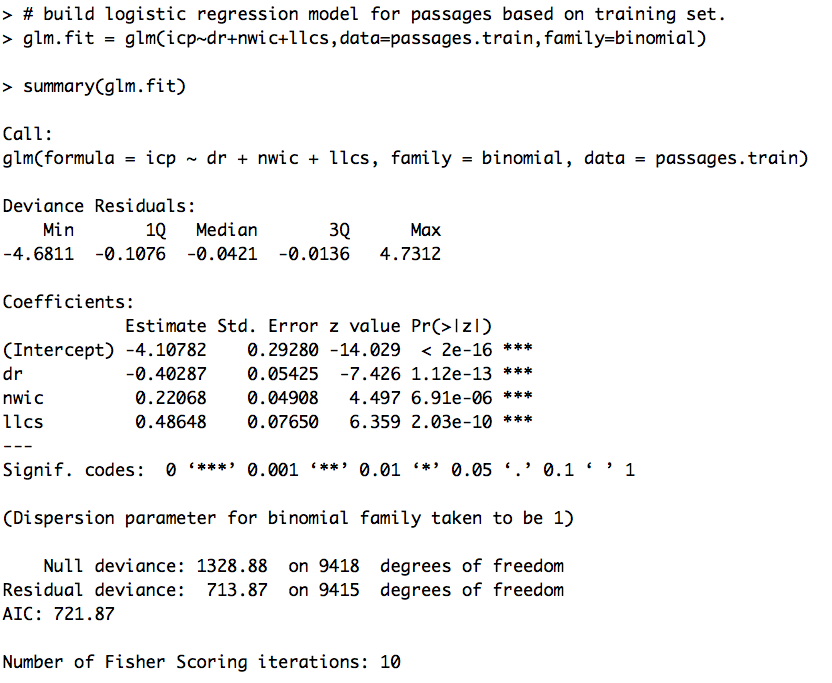
\includegraphics[width=125mm, height=125mm]{logit_model_summary.png}
\caption{Passage Classification Model Summary}
\label{fig:logistic_model_summary}
\end{figure}


\section{Application to the Test Set}

The application of the classification model to the passage test set yields favorable results.  Fig.~\ref{fig:logit_model_test_set_top} shows an extract of the data, where each record corresponds to a passage (whose text is not shown).  The fields show the question id to which the passage applies, the input variables, including dr, nwic, and llcs, and the output variable, icp.  On the far right is the relevance probability assigned by the model.  In this case, we're not so much interested in whether this value is less than or greater than 0.5, as is commonly the case in a logistic model, but instead, its relative magnitude compared with the probabilities of the other passages for the same question.  Fig.~\ref{fig:logit_model_test_set_top} shows the records for the top seven passages for five exam questions, ranked in order of decreasing probability for each question.  The reader will notice that for each question, the passage assigned the highest relevance probability is also, in fact, the correct passage, (icp = 1), with the exception of the first question.  In fact, the classification model correctly assigns the highest probability to the correct passage for 12 of the 16 questions.  And it omits the correct passage from its top seven passages (this number determined as reasonable from observation of the training set) for only one out of the collection of 16 test questions, as evidenced in Fig.~\ref{fig:test_set_correct_passage_count}.  In other words, its recall is 93\% using a capture size of seven.


\begin{figure}
\centering
\vspace{1.0in}
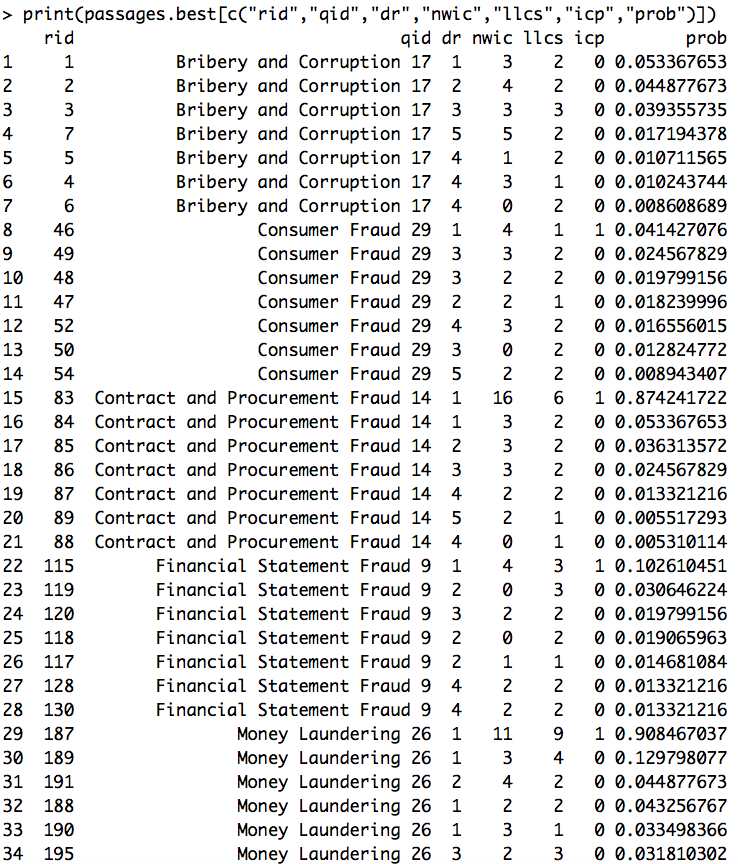
\includegraphics[width=125mm, height=125mm]{logit_model_test_set_top.png}
\caption{Application of the Passage Classification Model to the Test Set}
\label{fig:logit_model_test_set_top}
\end{figure}

\begin{figure}
\centering
\vspace{1.0in}
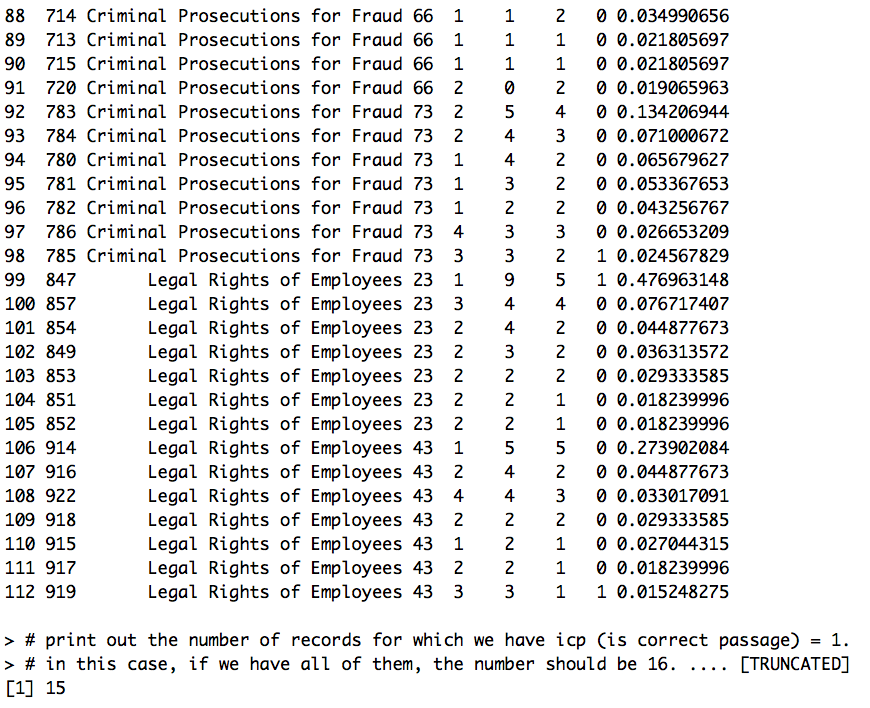
\includegraphics[width=125mm, height=125mm]{logit_model_test_set_bottom.png}
\caption{Test Set - Count of Correct Passages Retrieved By Classification Model}
\label{fig:test_set_correct_passage_count}
\end{figure}




\section{Answer Processing Algorithms for Version 3}

The answer processing algorithms discussed in this section leverage the top seven passages extracted using the passage classification logistic regression model.  Both of these algorithms are relatively straight-forward in nature and utilize the refined text body in a significant way.  

	% \subsection{Application of the Passage Selection Logit Model}



		% using lucene, as in chapter 04, to get likely documents, and 
		% the passages within 
		% them.
		
		% apply the logit model to determine the probability of being 
		% the correct passage for each passage among the likely documents.
		% rank the passages in order of decreasing probability.
		% select the top 7 passages.

		% \subsubsection{Performance of Passage Selection Logit Model}
		
\subsection{MLPassage1}

MLPassage1 essentially uses the same Max Joint Probability algorithm used in Version 1.  That is, this algorithm calculates the geometric mean frequency of the words in each answer option within the text body for the question.  Except this time, of course, the text body is much more refined to the question.  We see an example of MLPassage1 in Fig.~\ref{fig:mlpassage1_test_case_correct}, where this algorithm successfully selects the correct answer.  We also see its justification for its selection by virtue of the computations of the geometric mean and its selection of the option with the highest value.  However, we are also reminded in this justification that the text body on which it is performing these calculation results from a logistic regression model whose justification is, at best, opaque.  



\begin{figure}
\centering
\vspace{1.0in}
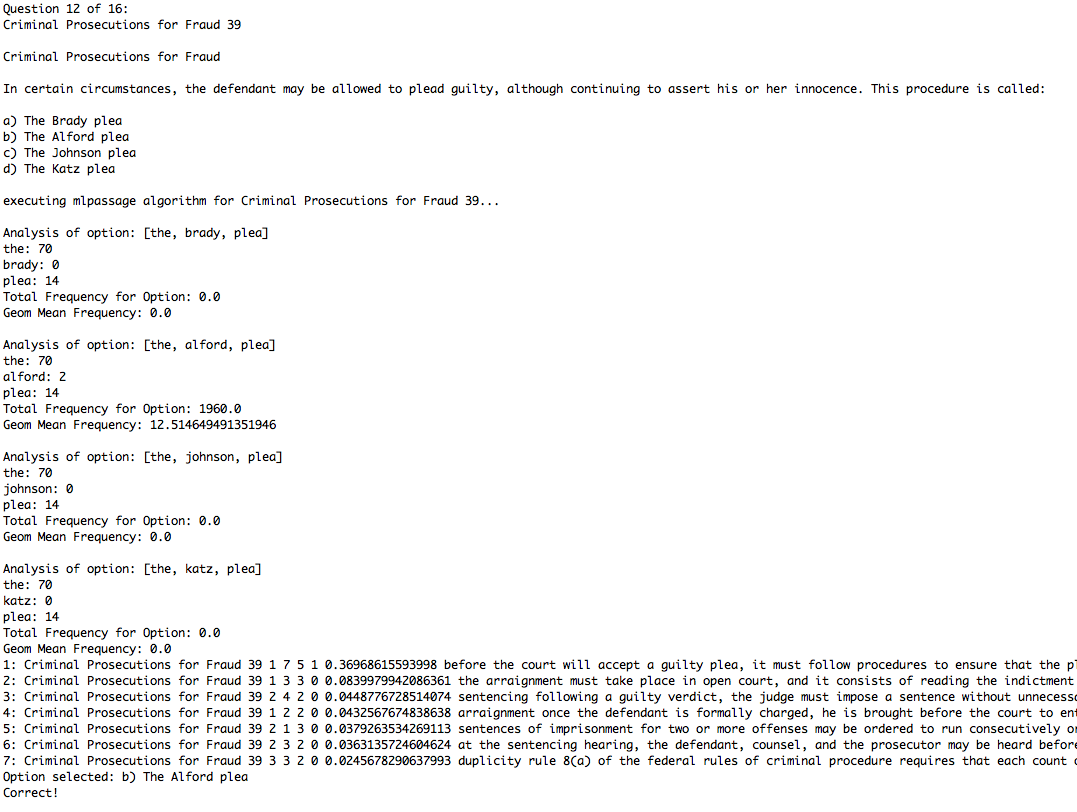
\includegraphics[width=125mm, height=125mm]{mlpassage1_test_case_correct.png}
\caption{MLPassage1 Algorithm - Test Case 1}
\label{fig:mlpassage1_test_case_correct}
\end{figure}

\subsubsection{MLPassage1 Performance}

For the test set of 16 questions, this algorithm answered 8 questions correctly, 50\%.  Despite the refined approach to selecting passages, this algorithm did not perform up to expectations.  Reasons for this are discussed below.


For a number of other questions in the test set, the algorithm failed to select the correct answer, as shown in the Fig.~\ref{fig:mlpassage1_test_case_incorrect}.  As shown in the answer justification, the problem here stems from the fact that because there is no smoothing (such as, Laplace smoothing) of word frequencies, those options with at least one word that does not occur in the narrowly focused text body are assigned a score of zero.  In the case of the example shown here, the word, ``scam" does not appear anywhere in the text body, and thus all options are assigned a score of zero since all of them include the word ``scam".  Other problems are made apparent in the test set, as well.  MLPassage1 also includes no stemming of the words in order to account for word transformations between the options and the text body.  

Finally, we must remember that only one of the passages is actually considered the correct passage among the seven passages extracted by the passage classification model.  The other six are, in fact, not relevant.  To the extent MLPassage1 includes all of the passages in its text body for each question, these other six may have a deleterious effect on the performance of the algorithm.  The next algorithm takes this phenomenon into account by using only the first passage among the seven (that is, the passage with highest probability of relevance).

\begin{figure}
\centering
\vspace{1.0in}
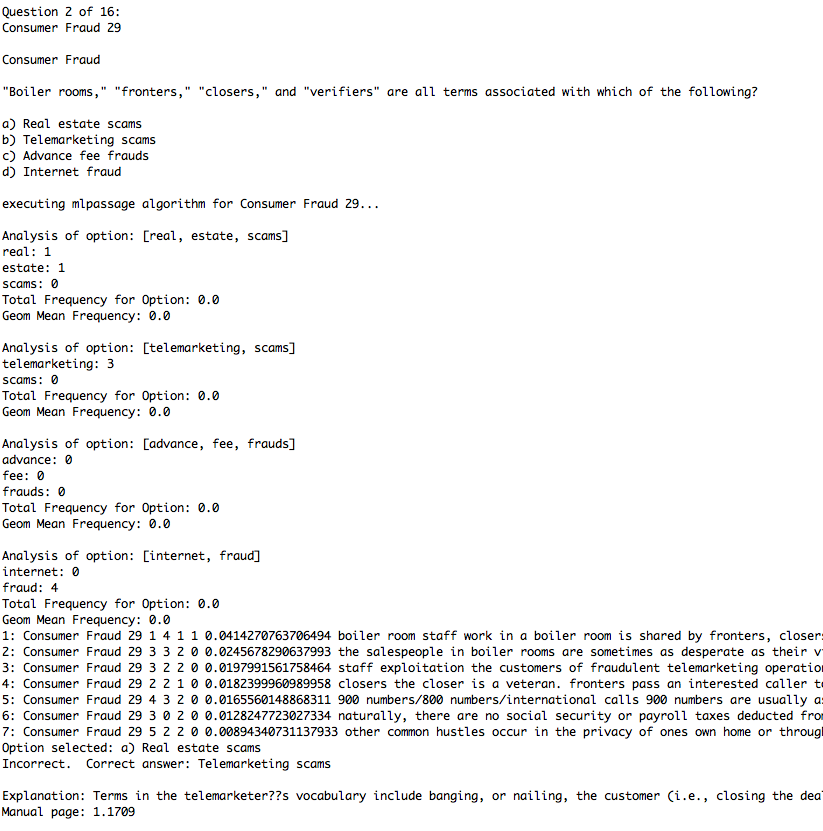
\includegraphics[width=125mm, height=125mm]{mlpassage1_test_case_incorrect.png}
\caption{MLPassage1 Algorithm - Test Case 2}
\label{fig:mlpassage1_test_case_incorrect}
\end{figure}


\subsection{MLPassage2}

MLPassage2 addresses two of the problems cited with MLPassage1, namely the stemming problem and the passage selection problem.  An implementation of the Porter Stemmer algorithm was incorporated into this algorithm to address the first issue.  As for the second, this algorithm includes only the first text passage out of the seven.  As noted above, the passage classification algorithm has good precision.  So, reducing the text body to only the first passage would appear to be a prudent decision.  The results bear this out -- With these modifications, the MLPassage2 algorithm shows improved performance of 11 of 16 correct (68.75\%), as shown in Fig.~\ref{fig:mlpassage2_performance}.  

The performance of MLPassage2 is comparable to that seen in Version 2 of the agent on definition questions.  There is more room for enhancements and modifications to MLPassage2, however, which should result in better performance with further research.

\begin{figure}
\centering
\vspace{1.0in}
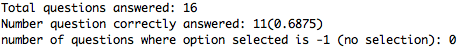
\includegraphics[width=50mm, height=10mm]{mlpassage2_performance.png}
\caption{MLPassage2 Algorithm Performance}
\label{fig:mlpassage2_performance}
\end{figure}





















